% !TEX TS-program = pdflatex
% !TEX encoding = UTF-8 Unicode

% Example of the Memoir class, an alternative to the default LaTeX classes such as article and book, with many added features built into the class itself.

%\documentclass[12pt,a4paper,article]{memoir} % for a short document
\documentclass[12pt,letterpaper]{memoir} % for a long document

\usepackage[utf8]{inputenc} % set input encoding to utf8
\usepackage{graphicx}

% Don't forget to read the Memoir manual: memman.pdf

%%% Examples of Memoir customization
%%% enable, disable or adjust these as desired

%%% PAGE DIMENSIONS
% Set up the paper to be as close as possible to both A4 & letter:
\settrimmedsize{11in}{8in}{*} % letter = 11in tall; a4 = 210mm wide
\setlength{\trimtop}{0pt}
\setlength{\trimedge}{\stockwidth}
\addtolength{\trimedge}{-\paperwidth}
\settypeblocksize{*}{\lxvchars}{1.618} % we want to the text block to have golden proportionals
\setulmargins{50pt}{*}{*} % 50pt upper margins
\setlrmargins{*}{*}{1.618} % golden ratio again for left/right margins
\setheaderspaces{*}{*}{1.618}
\checkandfixthelayout 
% This is from memman.pdf

%%% \maketitle CUSTOMISATION
% For more than trivial changes, you may as well do it yourself in a titlepage environment
\pretitle{\begin{center}\sffamily\huge\MakeUppercase}
\posttitle{\par\end{center}\vskip 0.5em}

%%% ToC (table of contents) APPEARANCE
\maxtocdepth{subsection} % include subsections
\renewcommand{\cftchapterpagefont}{}
\renewcommand{\cftchapterfont}{}     % no bold!

%%% HEADERS & FOOTERS
\pagestyle{ruled} % try also: empty , plain , headings , ruled , Ruled , companion

%%% CHAPTERS
\chapterstyle{hangnum} % try also: default , section , hangnum , companion , article, demo

\renewcommand{\chaptitlefont}{\Huge\sffamily\raggedright} % set sans serif chapter title font
\renewcommand{\chapnumfont}{\Huge\sffamily\raggedright} % set sans serif chapter number font

%%% SECTIONS
\hangsecnum % hang the section numbers into the margin to match \chapterstyle{hangnum}
\maxsecnumdepth{subsection} % number subsections

\setsecheadstyle{\Large\sffamily\raggedright} % set sans serif section font
\setsubsecheadstyle{\large\sffamily\raggedright} % set sans serif subsection font

%% END Memoir customization

\title{CGEM}
\author{Lisa L. Lowe}
%\date{} % Delete this line to display the current date

%%% BEGIN DOCUMENT
\begin{document}

\setverbatimfont{\normalfont\ttfamily}

\maketitle
\tableofcontents* % the asterisk means that the contents itself isn't put into the ToC

\chapter{Chapter 1}
\section{Section 1}
\subsection{Subsection 1}


\appendix

\chapter{Getting your Windows environment ready to use the HPC resources}



\section{Iris instructions for putty and remote host}

Download putty: 

\begin{verbatim}https://the.earth.li/~sgtatham/putty/latest/w64/putty.exe \end{verbatim}

Download and unzip Mobaxterm (portable home version, no installer): 
\begin{verbatim}http://download.mobatek.net/10220170312132617/MobaXterm_Portable_v10.2.zip\end{verbatim}

Run Mobaxterm, make sure “X server” is green:
\begin{center}
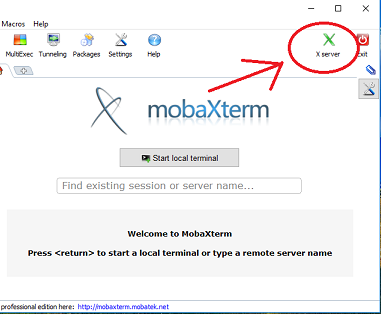
\includegraphics{Figures/App1/Env/Moba.PNG}
\end{center}


Set up putty (or atmos):

Host Name for iris: iris1.rtpnc.epa.gov

Host Name for atmos: atmost.nesc.epa.gov

Should look like this (and save your sessions once you set them up):
\begin{center}
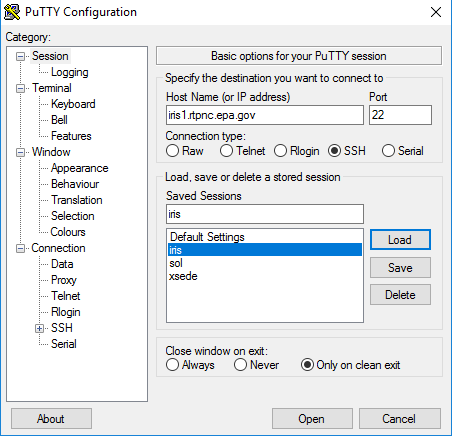
\includegraphics{Figures/App1/Env/putty_basic.PNG}
\end{center}

But before you log in by clicking “Open”, also set X-11 forwarding (and save!), Click on SSH then X11 then click the box to Enable X11 forwarding:
\begin{center}
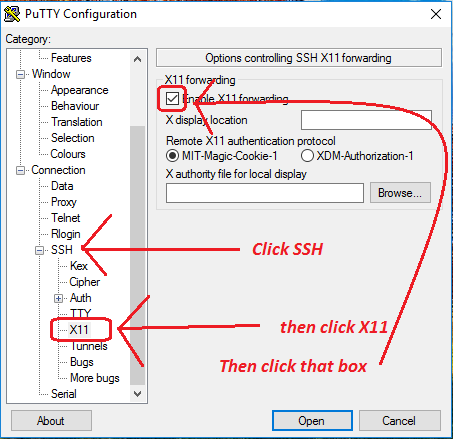
\includegraphics{Figures/App1/Env/X11.PNG}
\end{center}

Having X11 forwarding and also MobaXterm allows iris to open a window on your computer for things like opening emacs or a pdf file from iris without scp-ing it to your local machine.  But if it doesn’t work or is really slow and you can’t wait around, you can WinSCP the file to your local directory.  Email Rob McCauley for support if you have problems with remote display on iris.

\chapter{Using git and GitHub}

\section{Getting a GitHub account}

Go to github.com

\begin{center}
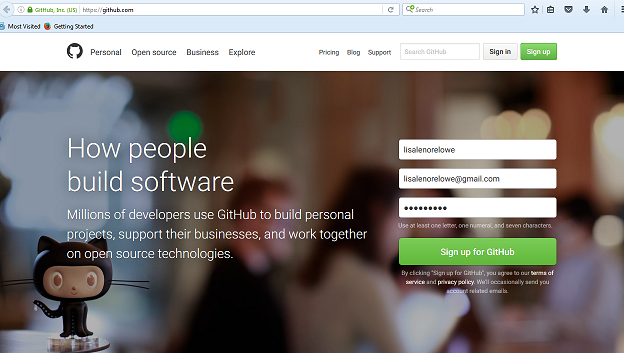
\includegraphics{Figures/App2/Git/GitHub_login.png}
\end{center}

Enter a user name, your email (use your EPA email address if you an EPA employee), and your password.

On the next page, choose “Unlimited public repositories for free” and click the green “continue” button.

You can answer the questions on the next page, or click “skip this step”.

Check your email, you will receive an email from github saying “Please verify your email address”. Click on the link to verify.

That’s it, you do not have to complete anything else.

To sign in again later, go back to the main page and click “Sign In” at the top right of the page.

Please email Lisa Lowe, 
\begin{verbatim} lowe.lisa@epa.gov\end{verbatim} 
with your github username and the associated email address, and it will be requested that you be given group permissions to the CGEM site: \begin{verbatim}https://github.com/USEPA/CGEM \end{verbatim}.



\end{document}
